To define the semantics of LCA, we formalize the intuitive notation of
the ancestor relationship between versions of a legal branching
history (i.e., a branching history generated by the rules in
Fig.~\ref{fig:opsem}):

\begin{definition} [\bfseries Ancestor]
Version $v_1$ is a ancestor of version $v_2$ under a history
$H$ (written $\under{H}{v_1 \preceq v_2}$) if and only if one of the
following is true:
\begin{itemize}
  \item There exists a branch $b$ in $H$ (i.e., $\exists(t\in
  dom(H)).\,H(t) = b$) in which $v_2$ immediately succeeds
  $v_1$,
  \item There exists a branch $b$ in $H$ that contains $(v_2, 
  \C{FORK}\; (v_1,f_1)::b_1)$, for some $f_1$ and $b_1$,
  \item There exists a branch $b$ in $H$ that contains
  $(v_2, \C{MERGE}\;(v_1,f_1)::b_1)$, for some $f_1$ and $b_1$,
  \item $v_1 = v_2$, or $v_1$ is transitively a ancestor of
  $v_2$, i.e., $\exists v.~ \under{H}{v_1 \preceq v} \conj
  \under{H}{v \preceq v}$ 
\end{itemize}
\end{definition}

The ancestor relation is therefore a partial order with a greatest
lower bound (the initial version).  Thus, for any two versions in a
legal history, there exists at least one common ancestor.  The ancestor
relationship among all common ancestors lets us define the notion of a
least common ancestor (LCA):

\begin{definition} [\bfseries Least Common Ancestor]
Version $v$ is said to be a common ancestor of versions $v_1$ and
$v_2$ under a history $H$ if and only if $\under{H}{v \preceq v_1}$
and $\under{H}{v \preceq v_2}$. It is said to be the least common
ancestor (LCA) of $v_1$ and $v_2$, iff there does not exist a $v'$
such that $\under{H}{v' \preceq v_1}$ and $\under{H}{v' \preceq v_2}$
and $\under{H}{v \preceq v'}$.
\end{definition}

When merging two concurrent versions $v_1$ and $v_2$, the common
ancestor argument for \C{merge} must be the LCA of $v_1$ and $v_2$,
without which \C{merge} may yield unexpected results. This is
demonstrated for the grow-only counter in
Fig.~\ref{fig:merge-needs-lca}, where an incorrect count is obtained if a
common ancestor that is not an LCA is used to merge 4 and 7. While in
this example there is a unique LCA for 4 and 7, in general this may
\begin{wrapfigure}{l}{.4\textwidth}
\centering
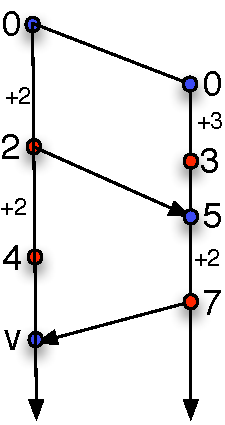
\includegraphics[scale=0.6]{Figures/merge-needs-lca}
\caption{This example of a grow-only counter illustrate why \C{merge}
needs a least common ancestor, and not just a common ancestor. Both 0
and 2 are common ancestors of 4 and 7, while 2 is their least common
ancestor (since $0 \preceq 2$). The result (v) of merging 4 and 7 is
11 (incorrect) if 0 is used as the common ancestor for merge, and 9
(correct, because 2+2+3+2 = 9) if 2 is used. }
\label{fig:merge-needs-lca}
\end{wrapfigure}
not be the case. With unrestrained branching and merging, there is no
bound on the number of LCAs a pair of versions can have.  For example,
in Fig.~\ref{fig:criss-cross-lcas}, the merge of 0 with 3 is preceded
by two ``criss-cross'' merges between their respective branches
resulting in there being two LCAs (5 and 4) for 0 and 3. Multiple LCAs
can occur even without criss-cross merges, as demonstrated by
Fig.~\ref{fig:external-lcas}. Concurrent versions with multiple LCAs
do not lend themselves to three-way merging. This problem also arises
in the context of source control systems, which employ \emph{ad hoc}
mechanisms to pave the way for three-way merging.
GitHub~\cite{github}, for instance, recursively merges LCAs to compute
a virtual ancestor, which then serves as the LCA for merging
concurrent versions. This method is demonstrated in the branching
structure for a mergeable, replicated counter as shown in
Fig.~\ref{fig:criss-cross-lcas}, where LCAs 5 and 4 of 0 and 3 are
merged (with their LCA being 10) to generate -1 as the virtual LCA to
merge 5 and 4. A major downside with this approach is that it makes no
guarantees on the relationship between the virtual ancestor and its
concurrent versions; the former may not even be a legal ancestor of
the latter as per the semantics of the data type. For instance,
suppose the integer type in Fig.~\ref{fig:criss-cross-lcas} represents
a bank account balance, which is expected to disallows any activity on
the account if the balance is ever known to be less than zero.  From
the perspective of the library designer and its clients, there is no
meaningful scenario in which versions 3 and 0 can emerge from -1,
since the only transition allowed by the semantics from -1 is to
itself.  Clearly, \emph{ad hoc} mechanisms like this are error-prone
and difficult to apply in general.

\begin{figure}[!t]
\centering
\subcaptionbox[] {\small
  In this example, 1 and 3 have two LCAs (3 and 4) a result of
  previous merges. The dotted circle denotes a virtual ancestor
  obtained by merging the two LCAs.
  \label{fig:criss-cross-lcas}
} [0.47\columnwidth] {
  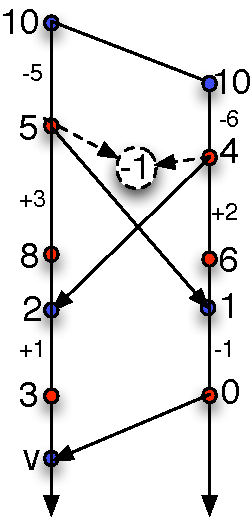
\includegraphics[scale=0.55]{Figures/2-LCAs}
}
\hfill
\subcaptionbox[] {\small
  In this example, versions $v_{13}$ and $v_{44}$ have two LCAs
  ($v_{22}$ and $v_{32}$)  despite there not being any previous merges
  between their respective branches.
  \label{fig:external-lcas}
} [0.47\columnwidth] {
  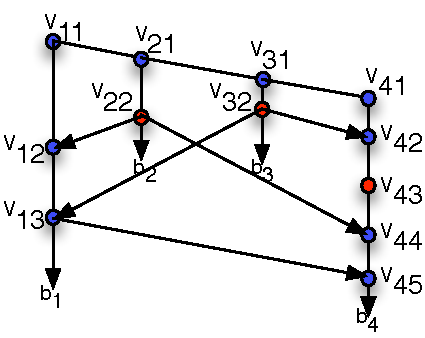
\includegraphics[scale=0.7]{Figures/2-external-LCAs}
}
\caption{Examples where merging versions have more than one LCA}
\label{fig:many-lcas}
\end{figure}


Fortunately, unlike source control systems where branching structure
is entirely dictated by the user, \name abstracts away branching
structure from the programmer, and hence retains the ability to
manifest it in a way that it deems fit. In particular, \name solves
the problem of multiple LCAs either by constraining the branching
stucture to prevent their existence, or by merging branches to ensure
that they have a new unique LCA.  Preention is done for
criss-cross merges by the operational semantics, which only allows
merging versions that are the latest on their respective branches. For
instance, suppose $v_{11}$ and $v_{21}$ are the latest versions on branches
$b_1$ and $b_2$, respectively. Merging $b_2$ into $b_1$ entails
merging $v_{21}$ into $v_{11}$ to generate version $v_{12}$ on $b_1$.
Now, merging $b_1$ into $b_2$ involves merging $v_{12}$, the latest
version on $b_1$, into $v_{21}$, but not $v_{11}$ into $v_{21}$, thus
preempting a criss-cross branching structure.
% In other words, a criss-cross branching structure is prevented due
% to the order among merges between conflicting branches introduced as
% a result of \rulelabel{E-Pull-Wait} being an atomic step. 

Next, for branching structures where a pair of branches (i.e., their
respective latest versions) have multiple externally-located LCAs, we
suitably extend the branching structure to generate a new single LCA.
 For instance, consider
the example in Fig.~\ref{fig:external-lcas}, where (latest versions
on) branches $b_1$ and $b_4$ have two externally-located LCAs
($v_{22}$ and $v_{32}$), hence cannot be merged. Mergeability can
however be reclaimed by extending the branching structure as shown in
Fig.~\ref{fig:legal-extension-1}. The extension is done by first
merging $b_3$ into $b_2$ to create version $v_{23}$ on $b_2$, then
merging $b_2$ into $b_1$ to create version $v_{14}$ on $b_1$, and
finally merging $b_2$ into $b_4$ to create version $v_{45}$ on
$b_4$. Observe that $b_1$ and $b_4$ now have a single LCA ($v_{23}$)
hence are now mergeable. Mergeability could also have been reclaimed
by adopting an alternative extension to the branching structure as
shown in Fig.~\ref{fig:legal-extension-2}.

\begin{figure}[!t]
\centering
\subcaptionbox[] {\small
  $b_3$ is merged into $b_2$ to create $v_{23}$ here.
  \label{fig:legal-extension-1}
} [0.47\columnwidth] {
  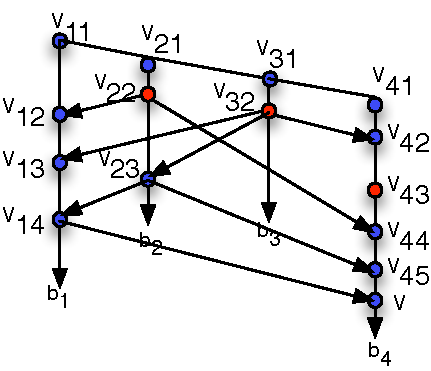
\includegraphics[scale=0.8]{Figures/legal-extension-1}
}
\hfill
\subcaptionbox[] {\small
  $b_2$ is merged into $b_3$ to create $v_{33}$ here.
  \label{fig:legal-extension-2}
} [0.47\columnwidth] {
  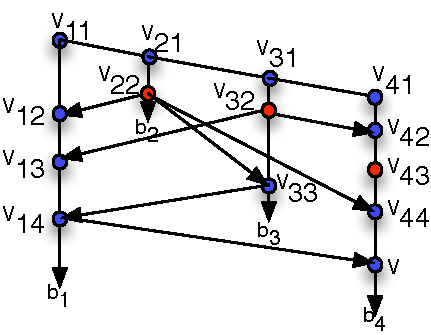
\includegraphics[scale=0.8]{Figures/legal-extension-2}
}
\caption{Legal extensions of the branching structure in
  Fig.~\ref{fig:external-lcas} that reclaim the mergeability of $b_1$
  and $b_4$}
\label{fig:legal-extensions}
\end{figure}


Note that the extension strategy described above is possible only
because operational semantics imposes no obligation to merge any two
concurrent versions. The high-level purpose of merging branches in
\name is to propagate the data across the branches, which can be done
by merging any two concurrent versions that contain the data; the
semantics lets us pick these versions. While mergeability of branches
with multiple LCAs can be reclaimed by actively extending the
branching structure as described above, the semantics is
\emph{self-correcting} in the sense that a fair execution reclaims the
mergeability of any two branches without any intervention. This is
possible because the system preempts criss-cross merges, thus letting
the semantics make progress from any state. The property is formalized
by the following theorem\footnote{The more precise statement of the
theorem, and its proof are included in the appendix}:

\begin{theorem} [\bfseries Semantics Self-Correcting]
??
\end{theorem}

The \rulelabel{E-Pull-Wait} uses the function \C{lca} to compute the
LCA of (the latest versions on) a pair of branches. The definition of
the function is standard, hence not discussed. 
